\section{Experiment}
\label{sec:experiment}

% 我们首先outline实验设置，包括模型，数据集和baselines，以及训练参数设计。
% 评估\ours在多个视觉幻觉相关的任务上的有效性。
% 进一步，我们分析\ours在不同类型的Vision任务上的泛化能力。
% 最后，我们进行消融研究，验证\ours中不同组件的贡献。

% % To thoroughly evaluate the effectiveness of \ours, 
% We first outline the experimental setup, the datasets, baselines, and training parameters. 
% We then assess \ours across diverse benchmarks.
% % Further, we analyze the generalization ability of \ours across different types of vision tasks.
% Finally, we conduct ablation studies to validate the contribution of different components.

The four functions in our method, $\text{Extract}(\vy)$, $\text{QA}(\vc_i)$, $\text{Ans}(\mI, \vv_i)$, and $\gF(\va_i,\, \va_i')$, are implemented via four distinct prompt templates. The details of templates are provided in Appendix~\ref{para:prompt_templates}.

\paragraph{Models, Datasets, and Baselines.}
% 我们评估\ours在Qwen2.5-VL的三个尺寸上（3B、7B、32B），以及Qwen3-VL的4B和8B版本上。
% 主实验中我们主要展示\ours在Qwen2.5-VL-7B上的结果，与其他baselines方法保持相同的模型规模，以确保公平比较。
% 9个baselines方法包括：BaseModel, 四个自进化的模型（不依赖图像的label/ground truth）包括：Vision-zero的三个版本（CLEVR、Chart、Real），EvoLMM，
% 四个模型（post-trained via RLVR on human-labeled data），R1-OneVision、VLAA-Thinker、MM-Eureka、OpenVLThinker。
% 训练数据集是32k的数据来自于GQA train数据集
% 评估的幻觉benchmarks 包括：AMBER, POPE, VSR-zeroshot, MME.
% 对于更多真实的多维度的评估，我们还在A-OKVQA, RealWorldQA, GQA(test), BLINK, NaturalBench, SEEDBench, MMMB, MMBench 等多个benchmark上进行全面评测。

We evaluate \ours on three sizes of Qwen2.5-VL (3B, 7B, and 32B)~\cite{qwen2p5vl}.
% as well as Qwen3-VL at 4B and 8B~\cite{qwen3vl}. 
For the main experiments, we primarily report results on Qwen2.5-VL-7B to ensure fair comparison with baselines at the same model scale.
% baselines
We compare against nine baselines across three categories:
(1) the \textbf{Base Model};
(2) four \textbf{self-evolving} models that require no ground-truth, including \textbf{Vision-Zero}~\cite{wang2026visionzero} (CLEVR, Chart, and Real) and \textbf{EvoLMM}~\cite{thawakar2025evolmm};
and (3) four models post-trained via RLVR on human-labeled data: \textbf{R1-OneVision}~\cite{yang2025r1}, \textbf{VLAA-Thinker}~\cite{chen2025vlaa}, \textbf{MM-Eureka}~\cite{meng2025mm}, and \textbf{OpenVLThinker}~\cite{deng2026openvlthinker}.
% benchmarks
For training, we sample 32K examples from the GQA training split~\cite{hudson2019gqa}. 
For evaluation, we report results on hallucination relevant benchmarks including AMBER~\cite{wang2023amber}, POPE~\cite{li2023pope}, VSR (zero-shot)~\cite{liu2023vsr}, and MME~\cite{fu2026mme}. 
To provide a more comprehensive assessment across capabilities, we further conduct extensive evaluation on A-OKVQA~\cite{schwenk2022okvqa}, RealWorldQA, GQA (test)~\cite{hudson2019gqa}, BLINK~\cite{fu2024blink}, NaturalBench~\cite{li2024naturalbench}, SEEDBench~\cite{li2024seedbench}, MMMB~\cite{sun2025mmmb}, and MMBench~\cite{liu2024mmbench}.
% 
We implement \ours using the Verl framework~\cite{sheng2024hybridflow}, and evaluate all models using the VLMEvalKit~\cite{duan2024vlmevalkit}.
We train with a learning rate of $2\times10^{-6}$, a batch size of 128, and a group size of 8.
The hyperparameters are selected heuristically: the deduplication threshold is set to $0.8$, $n_{\text{target}}=5$ for the claim quantity reward, and $\lambda_{\text{qual}}=0.1$ for the quality reward.
Further implementation details are provided in Appendix~\ref{sec:implementation_details}.

\subsection{Main Results}
% 我们与相同尺寸的9个baselines进行比较，加粗表示最佳结果，下划线表示第二好的结果。
% 首先评估了在hallucination相关的benchmark上的表现，见表1。
% 其次在 真实世界的VQA benchmark上评测\ours的表现，见表2。
% 最后在多个混合的全面的benchmark上进行评测，见表3。
% We compare \ours against nine baselines. Bold denotes the best result and underline denotes the second best.

% We first evaluate on different hallucination-related benchmarks in Table~\ref{tab:main_results}, followed by real-world visual question-answering benchmarks in Table~\ref{tab:main_results_vqa}, and finally conduct a comprehensive evaluation across multiple mixed benchmarks in Table~\ref{tab:main_results_mixed}.

% \begin{table*}[t]
% \centering
% \small
% \begin{tabular}{lcccccccccc}
% \toprule
%  & Qwen2.5-VL-7B & VisionZero(CLEVR) & VisionZero(Chart) & VisionZero(RealWorld) & EvoLMM & R1-Onevision & VLAA-Thinker & MM-Eureka & OpenVLThinker & Ours \\
% \midrule
% AMBER/Attribute  & 84.45 & 85.28 & 84.65 & 84.49 & 85.29 & 79.39 & 84.87 & 85.02 & 81.27 & 86.37 \\
% AMBER/ACC        & 85.01 & 86.19 & 84.86 & 85.11 & 85.60 & 82.61 & 85.17 & 85.04 & 83.96 & 88.48 \\
% AMBER/Existence  & 94.90 & 94.62 & 95.04 & 94.92 & 94.23 & 87.02 & 95.29 & 94.62 & 95.55 & 94.58 \\
% AMBER/Relation   & 75.66 & 78.67 & 74.88 & 75.90 & 77.28 & 81.43 & 75.36 & 75.48 & 75.06 & 84.50 \\
% GQA              & 60.46 & 60.61 & 60.28 & 60.35 & 60.59 & 0.00  & 60.34 & 60.25 & 9.75  & 60.92 \\
% MME/color        & 90.00 & 90.00 & 90.00 & 90.00 & 92.50 & 82.50 & 92.50 & 92.50 & 92.50 & 95.00 \\
% MME/existence    & 97.50 & 92.50 & 95.00 & 92.50 & 100.00 & 87.50 & 92.50 & 92.50 & 87.50 & 100.00 \\
% MME/position     & 82.50 & 82.50 & 82.50 & 80.00 & 81.67 & 60.83 & 85.00 & 82.50 & 75.00 & 86.67 \\
% POPE             & 86.51 & 86.78 & 86.23 & 86.41 & 87.29 & 82.42 & 86.19 & 85.71 & 79.25 & 87.04 \\
% VSR              & 90.64 & 91.96 & 90.82 & 90.21 & 91.35 & 72.73 & 90.52 & 90.91 & 86.12 & 92.03 \\
% \midrule
% Average          & 84.76 & 84.91 & 84.43 & 83.99 & 85.58 & 71.64 & 84.77 & 84.45 & 76.60 & 87.56 \\
% \bottomrule
% \end{tabular}
% \caption{Comparison results on multiple benchmarks.}
% \label{tab:main_results}
% \end{table*}
\begin{table*}[t]
\centering
\caption{
Performance comparison between \ours and baselines on multiple hallucination datasets.
AMBER evaluates attribute recognition, object existence, and spatial relation understanding.
MME assesses color, position, and scene perception.
POPE measures object hallucination, and VSR evaluates visual-spatial reasoning.
\textbf{Bold} denotes the best result and \underline{underline} denotes the second best.
$\Delta$ indicates the improvement over base model.
}
\label{tab:main_results}
\small
% \setlength{\tabcolsep}{4pt}
\begin{tabular}{l*{10}{S[table-format=2.2,table-column-width=0.8cm]}}
\toprule
 & \multicolumn{4}{c}{AMBER} & \multicolumn{3}{c}{MME} & \multicolumn{1}{c}{POPE} & \multicolumn{1}{c}{VSR} & \multicolumn{1}{c}{Avg.} \\

\cmidrule(lr){2-5}
\cmidrule(lr){6-8}
Method & \sh{Attribute} & \sh{Existence} & \sh{Relation} & \sh{Accuracy} & \sh{Color} & \sh{Position} & \sh{Scene} & {--} & {--} & {--} \\
\midrule

Qwen2.5-VL-7B         & 84.45 & 94.90 & 75.66 & 85.01 & 90.00 & 82.50 & 77.50 & 86.51 & 90.64 & 85.24 \\
VisionZero(CLEVR)     & 85.28 & 94.62 & 78.67 & \underline{86.19} & 90.00 & 82.50 & 79.00 & 86.78 & \underline{91.96} & \underline{86.11} \\
VisionZero(Chart)     & 84.65 & 95.04 & 74.88 & 84.86 & 90.00 & 82.50 & 77.50 & 86.23 & 90.82 & 85.16 \\
VisionZero(RealWorld) & 84.49 & 94.92 & 75.90 & 85.11 & 90.00 & 80.00 & 77.13 & 86.41 & 90.21 & 84.91 \\
EvoLMM                & \underline{85.29} & 94.23 & 77.28 & 85.60 & \underline{92.50} & 81.67 & \underline{79.75} & \textbf{87.29} & 91.35 & \underline{86.11} \\
R1-Onevision          & 79.39 & 87.02 & \underline{81.43} & 82.61 & 82.50 & 60.83 & 74.50 & 82.42 & 72.73 & 78.16 \\
VLAA-Thinker          & 84.87 & \underline{95.29} & 75.36 & 85.17 & {92.50} & \underline{85.00} & 77.13 & 86.19 & 90.52 & 85.78 \\
MM-Eureka             & 85.02 & 94.62 & 75.48 & 85.04 & {92.50} & 82.50 & 77.50 & 85.71 & 90.91 & 85.48 \\
OpenVLThinker         & 81.27 & \textbf{95.55} & 75.06 & 83.96 & {92.50} & 75.00 & 71.13 & 79.25 & 86.12 & 82.20 \\

\rowcolor{oursbg}
\midrule
\ours                  & \textbf{86.37} & 94.58 & \textbf{84.50} & \textbf{88.48} & \textbf{95.00} & \textbf{86.67} & \textbf{82.25} & \underline{87.04} & \textbf{92.03} & \textbf{88.54} \\
\rowcolor{oursbg}
$\Delta$ & \up{1.92} & \dn{0.32} & \up{8.84} & \up{3.47} & \up{5.00} & \up{4.17} & \up{4.75} & \up{0.53} & \up{1.39} & \up{3.30} \\
\bottomrule
\end{tabular}
\vspace{-3mm}
\end{table*}


\paragraph{Mitigating Hallucination.}
% paragraph 1: \ours 有效缓解多种类型的幻觉
Table~\ref{tab:main_results} reports results on hallucination-related benchmarks.
\ours achieves the best average score of 88.54, outperforming all baselines by a clear margin and improving over the base model by 3.30 points.
The gains are particularly pronounced in spatial and relational understanding: \ours improves Relation recognition by 8.84 points and Position perception by 4.17 points over the base model. The color dimension and attribute recognition also see substantial boosts of 5.0 and 1.92 points, respectively.
% , suggesting that our approach effectively addresses the systematic failures that vision-language models exhibit in fine-grained geometric reasoning.
% Notably, RLVR-based methods trained on human-labeled data (R1-OneVision, OpenVLThinker) show degraded performance relative to the base model on several metrics, indicating that indiscriminate supervision can introduce new hallucinations even while targeting other capabilities.
% In contrast, \ours consistently improves across nearly all dimensions without such side effects, with the sole exception of a marginal 0.32-point drop on Existence, which remains competitive.
These results demonstrate that \ours provides an effective and reliable approach to hallucination mitigation without ground-truth supervision.
% , without sacrificing accuracy on any specific perceptual dimension.

\paragraph{Strong Performance on Real-World VQA.}
% paragraph 2: \ours在多个VQA任务上表现出色
% Table~\ref{tab:main_results_vqa} reports results on open-ended VQA benchmarks.
In Table~\ref{tab:main_results_vqa}, \ours achieves the best performance on all three benchmarks, yielding an average score of 73.16 and surpassing the strongest baseline, EvoLMM, by 0.86 points.
The most substantial gain is observed on RealWorldQA (+3.53 over the base model), which requires grounded understanding of complex real-world visual scenes, suggesting that \ours develops more robust visual grounding beyond template-driven or synthetic training signals.
% Consistent improvements are also observed on A-OKVQA (+1.22) and GQA (+0.45), covering knowledge-grounded and compositional reasoning respectively, demonstrating the generality of our approach across diverse VQA paradigms.
% It is worth noting that R1-OneVision and OpenVLThinker exhibit near-zero scores on GQA, indicating severe format collapse under compositional reasoning tasks—a failure mode that \ours entirely avoids.
Taken together, these results confirm that \ours yields consistent and transferable improvements on real-world VQA without sacrificing generalization across task types.
\begin{wraptable}{r}{0.5\textwidth}
\centering
\vspace{-\intextsep}
\caption{
Performance comparison between \ours and baselines on multiple open-ended VQA benchmarks.
A-OKVQA (A-OK) evaluates knowledge-grounded visual question answering.
RealWorldQA (RWQA) measures understanding of real-world visual scenes QA.
% \textbf{Bold} denotes the best result and \underline{underline} denotes the second best.
% $\Delta$ indicates the improvement over base model.
}
\label{tab:main_results_vqa}
\small
\begin{tabular}{l*{4}{S[table-format=2.2,table-column-width=0.8cm]}}
\toprule
Method & {A-OK} & {GQA} & {RWQA} & {Avg.} \\
\midrule
Qwen2.5-VL-7B & 86.38 & 60.46 & 67.45 & 71.43 \\
VZ(CLEVR)     & 86.81 & \underline{60.61} & 67.97 & 71.80 \\
VZ(Chart)     & 85.76 & 60.28 & 67.97 & 71.34 \\
VZ(RealWorld) & 86.29 & 60.35 & 67.97 & 71.54 \\
EvoLMM        & \underline{86.90} & 60.59 & \underline{69.41} & \underline{72.30} \\
% R1-Onevision & 81.75 & 0.00 & 60.92 & 47.55 \\
VLAA-Thinker  & 85.68 & 60.34 & 65.49 & 70.50 \\
MM-Eureka     & 85.50 & 60.25 & 65.10 & 70.28 \\
% OpenVLThinker & 83.41 & 9.75 & 63.14 & 52.10 \\

\rowcolor{oursbg}
\midrule
\ours                  & \textbf{87.60} & \textbf{60.92} & \textbf{70.98} & \textbf{73.16} \\
\rowcolor{oursbg}
$\Delta$ & {\up{1.22}} & {\up{0.45}} & {\up{3.53}} & {\up{1.74}} \\
\bottomrule
\end{tabular}
\end{wraptable}


\paragraph{Comprehensive Gains on Multiple Mixed Benchmarks.}
\begin{table*}[t]
\centering
\caption{
Performance comparison between \ours and baselines on multiple mixed multi-task benchmarks.
% BLINK evaluates low-level visual perception including IQ test, jigsaw, multi-view reasoning, relative depth, and reflectance.
% NaturalBench measures compositional reasoning with overall accuracy, group, image, and question-level metrics.
% \textbf{Bold} denotes the best result and \underline{underline} denotes the second best.
% $\Delta$ indicates the improvement over base model.
}
\label{tab:main_results_mixed}
\small
\begin{adjustbox}{width=\textwidth}
\begin{tabular}{l*{13}{S[table-format=2.2,table-column-width=0.7cm]}}
\toprule
& MMB & MMMB & \multicolumn{5}{c}{BLINK} & \multicolumn{4}{c}{NaturalBench} & {SEED} & {Avg.} \\
\cmidrule(lr){4-8}
\cmidrule(lr){9-12}
Method & {--} & {--} & {IQ} & \sh{Jigsaw} & \sh{MVR} & \sh{Depth} & \sh{Rel.Refl.} & \sh{Acc} & \sh{G-Acc} & \sh{I-Acc} & \sh{Q-Acc} & {--} & {--} \\
\midrule

Qwen2.5-VL-7B & 80.62 & 82.83 & 0.67 & 46.67 & 33.83 & 71.77 & 29.85 & 77.97 & 31.79 & 60.39 & 57.89 & 76.36 & 54.22 \\
VZ(CLEVR)     & 80.99 & 82.93 & 1.33 & 51.33 & 24.06 & 70.97 & 27.61 & 78.18 & 32.58 & 60.76 & 58.37 & 76.48 & 53.80 \\
VZ(Chart)     & 80.16 & 82.98 & 0.67 & 36.67 & 32.33 & 69.35 & 22.39 & 78.09 & 31.63 & 60.50 & 58.03 & 76.48 & 52.44 \\
VZ(RealWorld) & 80.42 & 83.13 & 0.00 & 44.00 & \underline{39.85} & 73.39 & 27.61 & 78.08 & 32.26 & 60.50 & 58.18 & \underline{76.59} & 54.50 \\
EvoLMM        & 80.88 & \underline{83.48} & \underline{4.67} & \textbf{62.00} & 39.10 & \underline{75.00} & \underline{31.34} & 78.07 & 31.74 & 60.32 & 58.16 & 76.48 & \underline{56.77} \\
R1-Onevision  & 69.61 & 80.96 & 0.00 & 56.00 & 29.32 & 28.23 & 11.19 & 60.91 & 8.68 & 28.13 & 26.26 & 69.91 & 39.10 \\
VLAA-Thinker  & 80.10 & 82.27 & 1.33 & 35.33 & 20.30 & 71.77 & 28.36 & 78.33 & 32.84 & 61.08 & 58.66 & 76.54 & 52.24 \\
MM-Eureka     & 80.62 & 83.23 & 1.33 & 32.00 & 12.03 & 76.61 & 15.67 & 78.37 & \underline{33.00} & \textbf{61.29} & 58.71 & 76.42 & 50.77 \\
OpenVLThinker & 75.12 & 79.14 & 0.67 & \underline{56.67} & 20.30 & 51.61 & 20.15 & 66.59 & 16.95 & 37.95 & 36.42 & 72.25 & 44.48 \\

\midrule
\rowcolor{oursbg}
\ours          & \textbf{81.61} & \textbf{84.34} & \textbf{9.33} & \underline{56.67} & \textbf{41.35} & \textbf{79.03} & \textbf{38.06} & \textbf{78.53} & \textbf{33.32} & \underline{61.16} & \textbf{59.18} & \textbf{76.95} & \textbf{58.29} \\
\rowcolor{oursbg}
$\Delta$       & \up{0.99} & \up{1.52} & \up{8.67} & \up{10.00} & \up{7.52} & \up{7.26} & \up{8.21} & \up{0.55} & \up{1.53} & \up{0.76} & \up{1.29} & \up{0.59} & \up{4.07} \\
\bottomrule
\end{tabular}
\end{adjustbox}
\vspace{-2mm}
\end{table*}

% paragraph 3: \ours在多个综合评测benchmark上表现出色
Table~\ref{tab:main_results_mixed} presents results across a diverse set of general-purpose benchmarks spanning low-level visual perception, compositional reasoning, multi-image understanding, and holistic multimodal understanding.
\ours achieves the highest average score of 58.29, surpassing the previous best (EvoLMM, 56.77) by 1.52 points and improving over the base model by 4.07 points.
% The most striking gains emerge on BLINK, which probes low-level visual perception skills that are rarely targeted by existing training paradigms.
In BLINK, \ours 
% improves over the base model by 8.67 points on IQ Test, 10.00 points on Jigsaw, 7.52 points on Multi-View Reasoning, 7.26 points on Relative Depth, and 8.21 points on Reflectance—
achieves the best or second-best score on all five subtasks.
% These substantial and consistent improvements suggest that \ours cultivates genuine perceptual reasoning capabilities rather than merely adapting to benchmark-specific patterns.
On NaturalBench, which evaluates compositional reasoning through stringent group-, image-, and question-level accuracy, \ours again leads overall with improvements across all four metrics.
On the broader benchmarks MMBench and MMBench-Multi, \ours achieves scores of 81.61 and 84.34, respectively, along with the highest SEEDBench score of 76.95, demonstrating well-rounded capability across standard multimodal evaluation suites.
% In contrast, RLVR-based methods such as R1-OneVision and OpenVLThinker exhibit severe performance degradation on structurally complex tasks (e.g., R1-OneVision drops to 8.68 on G-Acc and 0.00 on IQ Test), further highlighting the robustness advantage of \ours.

\subsection{Model Generalization}
\label{sec:generalization}

\paragraph{Consistent gains across all scales.}
\begin{wrapfigure}{r}{0.5\textwidth}
    \centering
    \vspace{-\intextsep}
    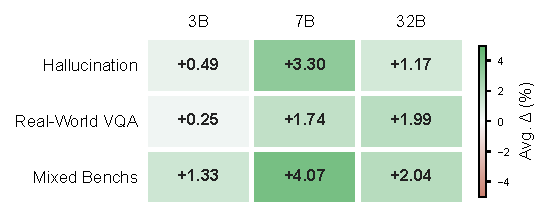
\includegraphics[width=0.48\textwidth]{figures/model_generalization_final_heatmap.pdf}
    \caption{Average improvements ($\Delta\%$) of \ours over the Qwen2.5-VL base model across three model scales and three benchmark categories. All cells are positive, demonstrating consistent gains at every scale.}
    \label{fig:model_gen_heatmap}
\end{wrapfigure}
To evaluate whether \ours generalizes across model scales, we apply the identical training recipe to Qwen2.5-VL-3B and 32B without any scale-specific modifications, and measure per-metric improvements relative to the respective base models.
As summarized in Figure~\ref{fig:model_gen_heatmap}, every cell of the $3{\times}3$ grid is positive, demonstrating that the claim-level self-verification signal benefits models regardless of capacity.
% The 7B model achieves the largest average gains ($+3.30$ on Hallucination, $+1.74$ on VQA, $+4.07$ on Mixed), consistent with the main results.
The 32B model improves substantially across all three categories ($+1.17$, $+1.99$, $+2.04$), with particularly strong per-metric gains of $+5.00$ on both MME/Color and MME/Position shown in Figure~\ref{fig:model_gen_bars}.
Even the 3B model benefits consistently: it achieves $+8.67$ on BLINK/Jigsaw and $+2.52$ on VSR zero-shot, yielding a $+1.33$ average improvement on Mixed benchmarks.
% The Mixed category consistently shows the largest average gain across all three model sizes ($+1.33$, $+4.07$, and $+2.04$ for 3B, 7B, and 32B, respectively).
% This pattern suggests that the fine-grained visual reasoning skills cultivated by claim-level self-verification transfer broadly to low-level perception, compositional reasoning, and holistic multimodal tasks—well beyond the hallucination domain targeted during training.
These results confirm that \ours generalizes reliably from 3B to 32B, without any scale-specific adaptations.

\begin{figure*}[t]
    \centering
    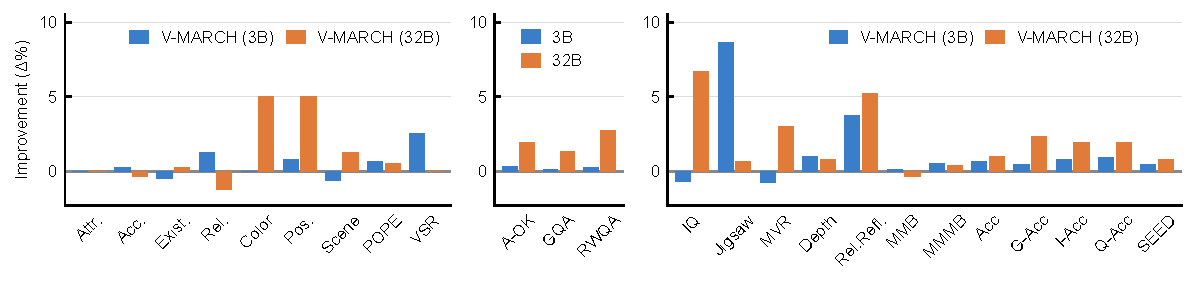
\includegraphics[width=\linewidth]{figures/model_generalization_final_bars.pdf}
    \vspace{-10mm}
    \caption{Per-metric performance improvements ($\Delta\%$) of \ours over the respective Qwen2.5-VL-3B and Qwen2.5-VL-32B base models, across (a) Hallucination, (b) Real-World VQA, and (c) Mixed Benchmarks.}
    \label{fig:model_gen_bars}
    \vspace{-3mm}
\end{figure*}


\subsection{Ablation Studies}

% \paragraph{Image Augmentation.}
% % 我们的方法考虑了actor生成时进行图像增强，来提升模型的鲁棒性和泛化能力。
% % 构建消融实验来验证图像增强的贡献，比较\ours与和不使用图像增强的版本在多个benchmark上的表现。
% To improve the model's robustness and generalization under diverse visual conditions, \ours incorporates stochastic image augmentation during actor rollout generation.
% We conduct an ablation study to quantify its contribution by comparing \ours against a variant trained without any image augmentation (\textit{w/o aug}) across all three benchmark categories.
% % 
% As shown in Table~\ref{tab:ablation_aug}, removing image augmentation leads to consistent performance drops across all three categories: $-0.58$ on Hallucination, $-0.98$ on Real-World VQA, and $-1.13$ on Multi-Task benchmarks.
% % The largest degradation is observed on the Multi-Task suite, suggesting that augmentation is particularly beneficial for benchmarks requiring robust low-level visual perception and compositional reasoning.
% % Notably, both \ours and its ablated variant still outperform the base model, confirming that the overall training framework is effective on its own; however, image augmentation provides a consistent and complementary boost across all evaluation dimensions.
% These results validate the design choice of applying augmentation during rollout, where diverse visual inputs encourage the model to develop more stable and generalizable visual representations rather than overfitting to a fixed image distribution.

% \begin{table}[t]
\centering
\caption{
% Overall comparison and ablation summary across three benchmark categories.
Ablation on the image augmentation module.
$\Delta$ denotes the improvement over the base model.
``Decrease'' denotes the performance drop compared with \ours after removing the augmentation module.
}
\label{tab:ablation_aug}
\small
\begin{adjustbox}{width=\linewidth}
\begin{tabular}{l*{3}{S[table-format=2.2,table-column-width=1.4cm]}}
\toprule
Method & {Hallucination} & {VQA(s)} & {Mixed(s)} \\
\midrule
% Qwen2.5-VL-7B & 85.24 & 71.43 & 54.22 \\
% \rowcolor{oursbg}
\ours & \textbf{88.54} & \textbf{73.16} & \textbf{58.29} \\
% \rowcolor{oursbg}
$\Delta$ & \up{3.30} & \up{1.74} & \up{4.07} \\
% \midrule
{--- w/o aug} & 87.97 & 72.19 & 57.16 \\
$\Delta$ & \up{2.73} & \up{0.76} & \up{2.94} \\
\midrule
\cellcolor{gray!10}Decrease & \negcell{-0.58} & \negcell{-0.98} & \negcell{-1.13} \\
\bottomrule
\end{tabular}
\end{adjustbox}
\end{table}


\paragraph{VCR Analysis.}
% \begin{table}[t]
% \centering
% \caption{
% Ablation study of different strategies.
% }
% \label{tab:ablation_com}
% \small
% \begin{tabular}{l*{3}{S[table-format=2.2,table-column-width=0.9cm]}}
% \toprule
% Method & {Hallucination} & {Real-World} & {Multi-Task} \\
% \midrule
% \ours                  & \textbf{88.54} & \textbf{73.16} & \textbf{58.29} \\
% \midrule
% \ours-nodedup          & 86.63 & 72.03 & 57.86 \\
% Decrease               & {\dn{1.92}} & {\dn{1.13}} & {\dn{0.43}} \\
% \midrule
% \ours-nocount          & 86.83 & 71.53 & 55.45 \\
% Decrease               & {\dn{1.71}} & {\dn{1.63}} & {\dn{2.85}} \\
% \midrule
% \ours-noquality        & 87.83 & 72.30 & 57.01 \\
% Decrease               & {\dn{0.71}} & {\dn{0.87}} & {\dn{1.28}} \\
% \bottomrule
% \end{tabular}
% \end{table}

\begin{wraptable}{r}{0.5\textwidth}
\centering
\vspace{-\intextsep}
\caption{
Ablation study of the VCR: claim deduplication (Dedup.), claim quantity reward ($r^{\text{cnt}}$), and claim quality penalty ($r^{\text{qual}}$).
Each variant removes one component at a time; Decrease denotes the performance drop relative to the full \ours method.
% All three components contribute positively, with $R_{\text{cnt}}$ yielding the largest overall gain and Dedup.\ proving most critical for hallucination mitigation.
}
\label{tab:ablation_com}
\small
\begin{tabular}{l*{3}{S[table-format=2.2,table-column-width=1.4cm]}}
\toprule
Method & {Hallucination} & {VQA(s)} & {Mixed(s)} \\
\midrule
\ours                  & \textbf{88.54} & \textbf{73.16} & \textbf{58.29} \\
\midrule
{--- w/o Dedup.}          & 86.63 & 72.03 & 57.86 \\
\cellcolor{gray!10}Decrease               & {\negcell{-1.92}} & {\negcell{-1.13}} & {\negcell{-0.43}} \\
\midrule
{--- w/o $r^{\text{cnt}}$}       & 86.83 & 71.53 & 55.45 \\
\cellcolor{gray!10}Decrease               & {\negcell{-1.71}} & {\negcell{-1.63}} & {\negcell{-2.85}} \\
\midrule
{--- w/o $r^{\text{qual}}$}        & 87.83 & 72.30 & 57.01 \\
\cellcolor{gray!10}Decrease               & {\negcell{-0.71}} & {\negcell{-0.87}} & {\negcell{-1.28}} \\
\bottomrule
\end{tabular}
\end{wraptable}

To assess the contribution of each VCR component, we ablate them individually and report results in Table~\ref{tab:ablation_com}.
\textbf{Dedup.}\ proves most critical for the Hallucination benchmark ($-1.92$): without semantic deduplication, the model exploits near-identical claims to inflate the consistency reward without genuinely improving perceptual accuracy, a form of reward hacking that degrades grounded perception.
\textbf{$r^{\mathrm{cnt}}$}\ exerts the broadest influence, yielding the largest drops on Mixed ($-2.85$) and notable degradation on Real-World VQA ($-1.63$) and Hallucination ($-1.71$); this pattern suggests that incentivizing sufficient claim diversity is essential for comprehensive visual coverage across task types.
\textbf{$r^{\mathrm{qual}}$}\ produces comparatively modest but consistent declines across all three categories ($-0.71$, $-0.87$, $-1.28$), confirming its complementary role in steering the Solver away from image-agnostic claims toward genuinely visually grounded responses.
Taken together, these results demonstrate that each VCR component addresses a distinct failure mode, and their combination is necessary for robust, reward-stable training.
Overall, all three components contribute positively and consistently, with claim quantity yielding the largest overall gain and claim deduplication being most critical for hallucination mitigation.

\paragraph{Granularity of Self-Verification.}

\begin{wraptable}{r}{0.5\textwidth}
\centering
\vspace{-\intextsep}
\caption{
Comparison of claim-level and response-level self-verification on the three benchmark categories.
Decrease denotes the performance drop to the claim-level.
}
\label{tab:claim_vs_response}
\small
% \begin{tabular}{lccc}
\begin{tabular}{l*{3}{S[table-format=2.2,table-column-width=1.4cm]}}
\toprule
Method & {Hallucination} & {VQA(s)} & {Mixed(s)} \\
\midrule
Claim-Level           & \textbf{88.54} & \textbf{73.16} & \textbf{58.29} \\
Response-Level  & 87.70 & 72.51 & 56.99 \\
\midrule
\cellcolor{gray!10}Decrease        & \negcell{-0.84} & \negcell{-0.66} & \negcell{-1.30} \\
\bottomrule
\end{tabular}
\end{wraptable}

A key design choice in \ours is the use of \textit{claim-level} self-verification.
% , which decomposes a model-generated caption into atomic, verifiable claims and checks each one independently against the image.
% As an alternative, \textit{response-level} verification directly scores the entire model output as a whole.
To empirically validate the superiority of our decomposed approach, we implement a response-level baseline that replaces the multi-stage claim pipeline.
Further implementation details are provided in Appendix~\ref{sec:response_level_self_verification}.
As shown in Table~\ref{tab:claim_vs_response}, claim-level verification consistently outperforms its response-level counterpart across all three benchmark categories.
% The largest gap appears on the Multi-Task suite ($-1.30$), where fine-grained perceptual tasks such as IQ Test ($-6.00$), Relative Depth ($-4.03$), and Multi-View Reasoning ($-3.76$) suffer most from the coarser holistic signal.
% On the Hallucination benchmarks, claim-level verification yields a $-0.84$ average advantage, with notable improvements in Existence ($-1.60$) and Relation ($-1.32$) recognition—precisely the attribute types that require targeted, per-claim scrutiny rather than global impression matching.
% On Real-World VQA, the gap is smaller ($-0.66$) but consistent, with RealWorldQA showing the sharpest drop ($-1.83$).
These results demonstrate that decomposing verification into atomic claims enables more precise reward signals during training, leading to more hallucination-resistant models.
% : errors in individual attributes are surfaced and penalized directly, whereas a holistic judge may overlook fine-grained mistakes when the overall description appears plausible.
% Claim-level verification provides a stronger and more reliable training signal, leading to better-calibrated and more hallucination-resistant models.

\paragraph{Training Dynamics.}
\begin{wrapfigure}{r}{0.5\textwidth}
    \centering
    \vspace{-\intextsep}
    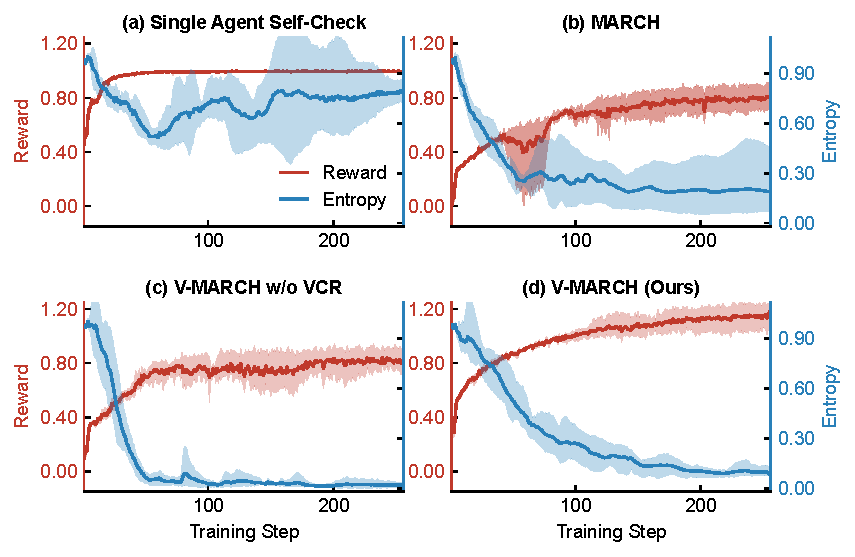
\includegraphics[width=0.48\textwidth]{figures/training_dynamics_2.pdf}
    \caption{Reward (red, left axis) and entropy (blue, right axis) curves over 256 training steps for (a) Single Agent SelfCheck, (b) MARCH~\cite{li2026march}, (c) V-MARCH w/o VCR, and (d) \textbf{\ours}. The comparison demonstrates that claim-level verification with VCR is necessary for stable, non-degenerate training.}
    \label{fig:training-dynamics}
\end{wrapfigure}

% Figure~\ref{fig:training-dynamics} examines training stability across three configurations to isolate the contribution of VCR.
% Single Agent Self-Check achieves rapid early reward gains but exhibits persistent entropy oscillation between 0.6 and 1.0, a signature of reward hacking under a coarse holistic verification signal.
% Removing VCR from V-MARCH eliminates this instability at a steep cost: entropy collapses to near 0.01 within the first half of training, indicating severe mode collapse and the loss of any meaningful exploration.
% The full V-MARCH pipeline produces monotonically increasing reward alongside a controlled entropy decrease that remains above 0.1 throughout, reflecting genuine policy improvement rather than degenerate exploitation.
% This training-time stability, enabled by the claim quantity reward $R_{\mathrm{cnt}}$ and quality penalty $R_{\mathrm{qual}}$ of VCR, translates directly into the performance advantage observed across all benchmark categories.

Figure~\ref{fig:training-dynamics} compares training stability across four configurations in a $2{\times}2$ analysis designed to isolate the contributions of VCR and claim-level reward structure.
% Single Agent SelfCheck accrues reward rapidly but never stabilizes, with entropy oscillating between 0.6 and 1.0 throughout all 256 steps---a clear signature of reward hacking induced by a coarse holistic verification signal.
% MARCH improves monotonically from $-0.01$ to ${\approx}0.81$ in reward, yet entropy plummets aggressively to 0.19, confirming that length-based surrogates suppress exploration beyond what is necessary for policy refinement.
% Removing VCR from \ours is more destructive still: reward growth becomes erratic and entropy collapses to near 0.01 within the first half of training, indicating degenerate convergence to a single repetitive strategy.
\ours pipeline is the only configuration that achieves both monotonically increasing reward and controlled entropy decay above 0.1, reflecting genuine policy improvement rather than exploitative shortcutting.
This training-time stability, conferred by the claim quantity reward $r^{\mathrm{cnt}}$ and quality penalty $r^{\mathrm{qual}}$ of VCR, directly underlies the performance advantage \ours demonstrates across all benchmarks.

\paragraph{Computational Overhead.}
% Our pipeline introduces additional inference overhead relative to single-agent baselines.
Table~\ref{tab:overhead} reports the wall-clock time per training step for each method.
EvoLMM~\cite{thawakar2025evolmm} trains separate Proposer and Solver models, and the switching overhead more than doubles the average step time compared to SelfCheck.
We therefore report a conservative estimate of twice the SelfCheck cost, which lower-bounds its true training overhead.
\ours comprises four agents, with only the Solver being trainable and the other three (Proposer, Regulator, Checker) frozen.
This design results in a per-step runtime of 281.21,s, representing a $1.56\times$ overhead compared to SelfCheck (180.02,s).
Given that \ours achieves consistent and substantial performance gains across all evaluation dimensions, this overhead represents a favorable trade-off between compute cost and reward quality.
\begin{table}[h]
\centering
\caption{Wall-clock time per training step, along with agent configuration \#Agent(trained/total) and relative overhead compared to SelfCheck with Ground Truth.}
\label{tab:overhead}
\begin{tabular}{lccc}
\toprule
\textbf{Method} & \textbf{Time / Step (s)} & \textbf{\#Agents} & \textbf{Overhead} \\
\midrule
SelfCheck (GT) & 171.24 & 1/2 & $\times1.00$ \\
SelfCheck      & 180.02 & 1/2 & $\times1.05$ \\
EvoLMM*      & 360.04 & 2/2 & $\times2.10$ \\
\rowcolor{oursbg}
\ours          & 281.21 & 1/4 & $\times1.56$ \\
\bottomrule
\end{tabular}
\end{table}

% \paragraph{Training Dynamics and Efficiency.}
% % 我们分析\ours的训练动态，包括训练中的reward曲线，entropy变化情况，以及训练的overhead。
% % - reward 曲线：评估\ours在训练过程中提供的奖励信号的稳定性和有效性，验证模型是否能够持续获得正向反馈并逐步提升性能。
% % - Entropy convergence: 评估模型输出的多样性和不确定性，验证\ours在训练过程中能够引导模型逐渐收敛到更准确和稳定的输出分布。
% % - overhead，wall-clock time: 评估\ours在训练过程中引入的额外计算开销，并与其他方法进行比较.

% \begin{figure}[htbp]
%     \centering
%     \begin{subfigure}{0.57\linewidth}
%         \centering
%         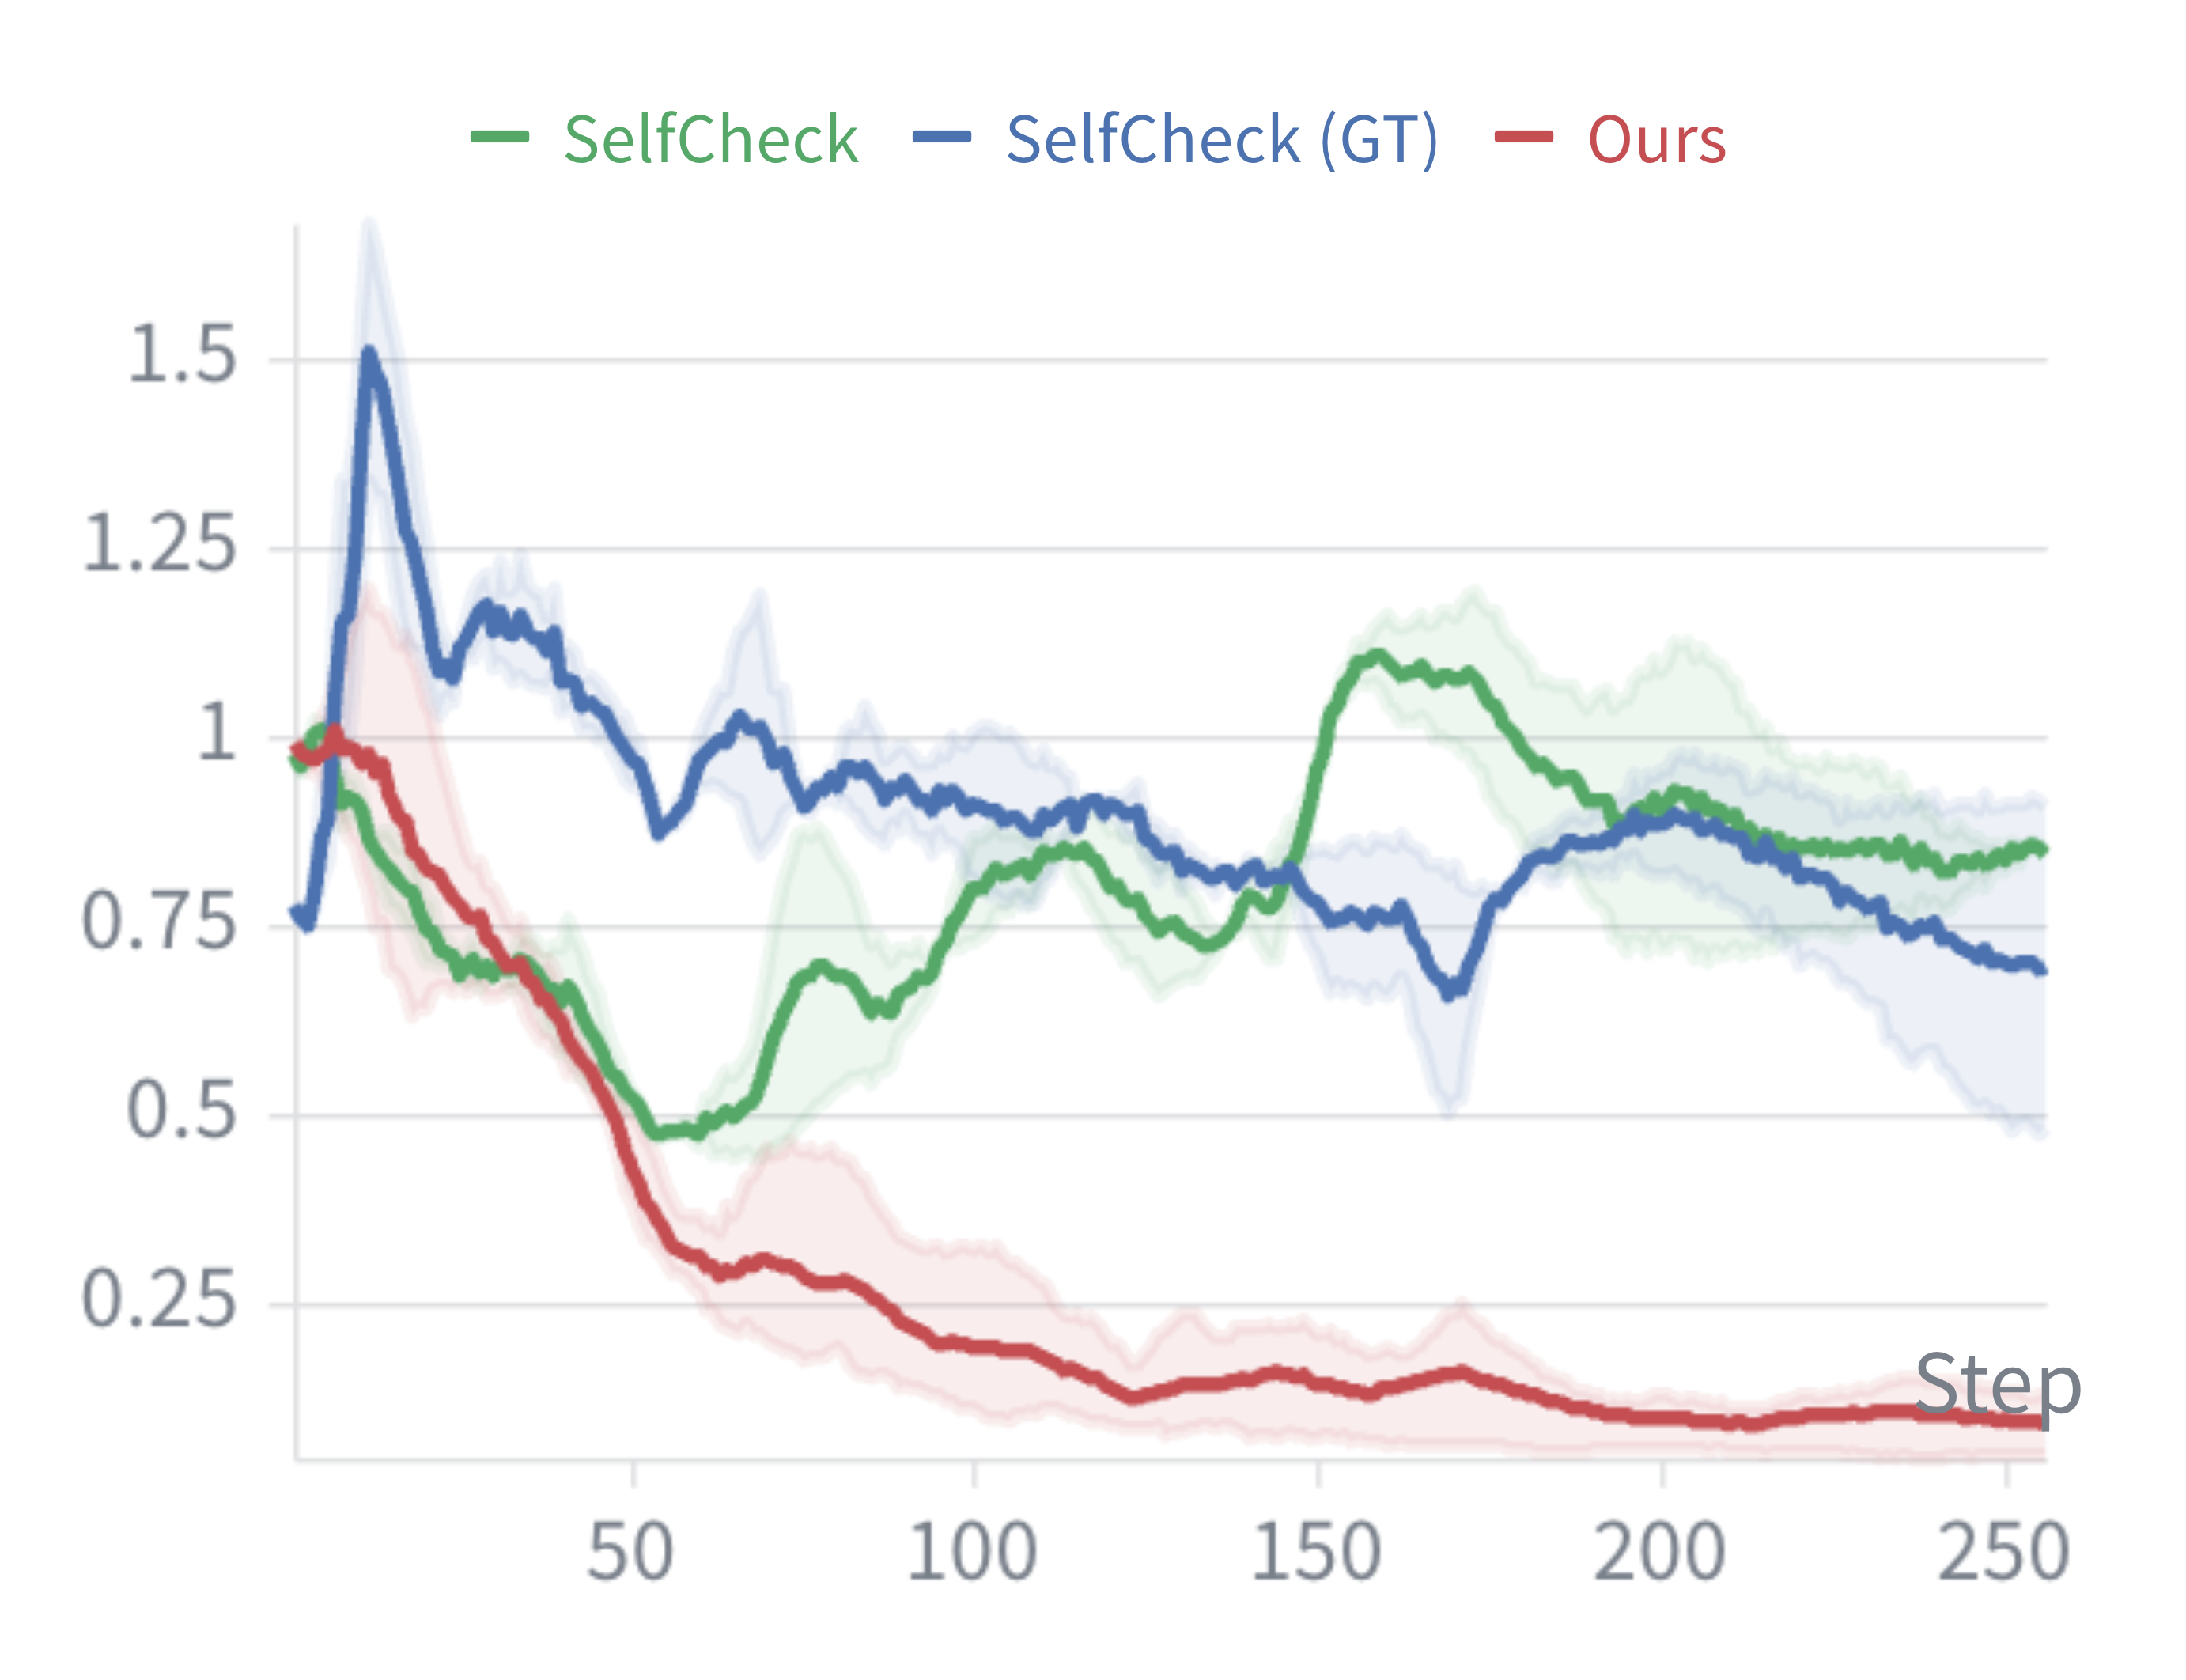
\includegraphics[width=\linewidth]{figures/vlmarch-entropy-2.png}
%     \end{subfigure}
%     \hfill
%     \begin{subfigure}{0.41\linewidth}
%         \centering
%         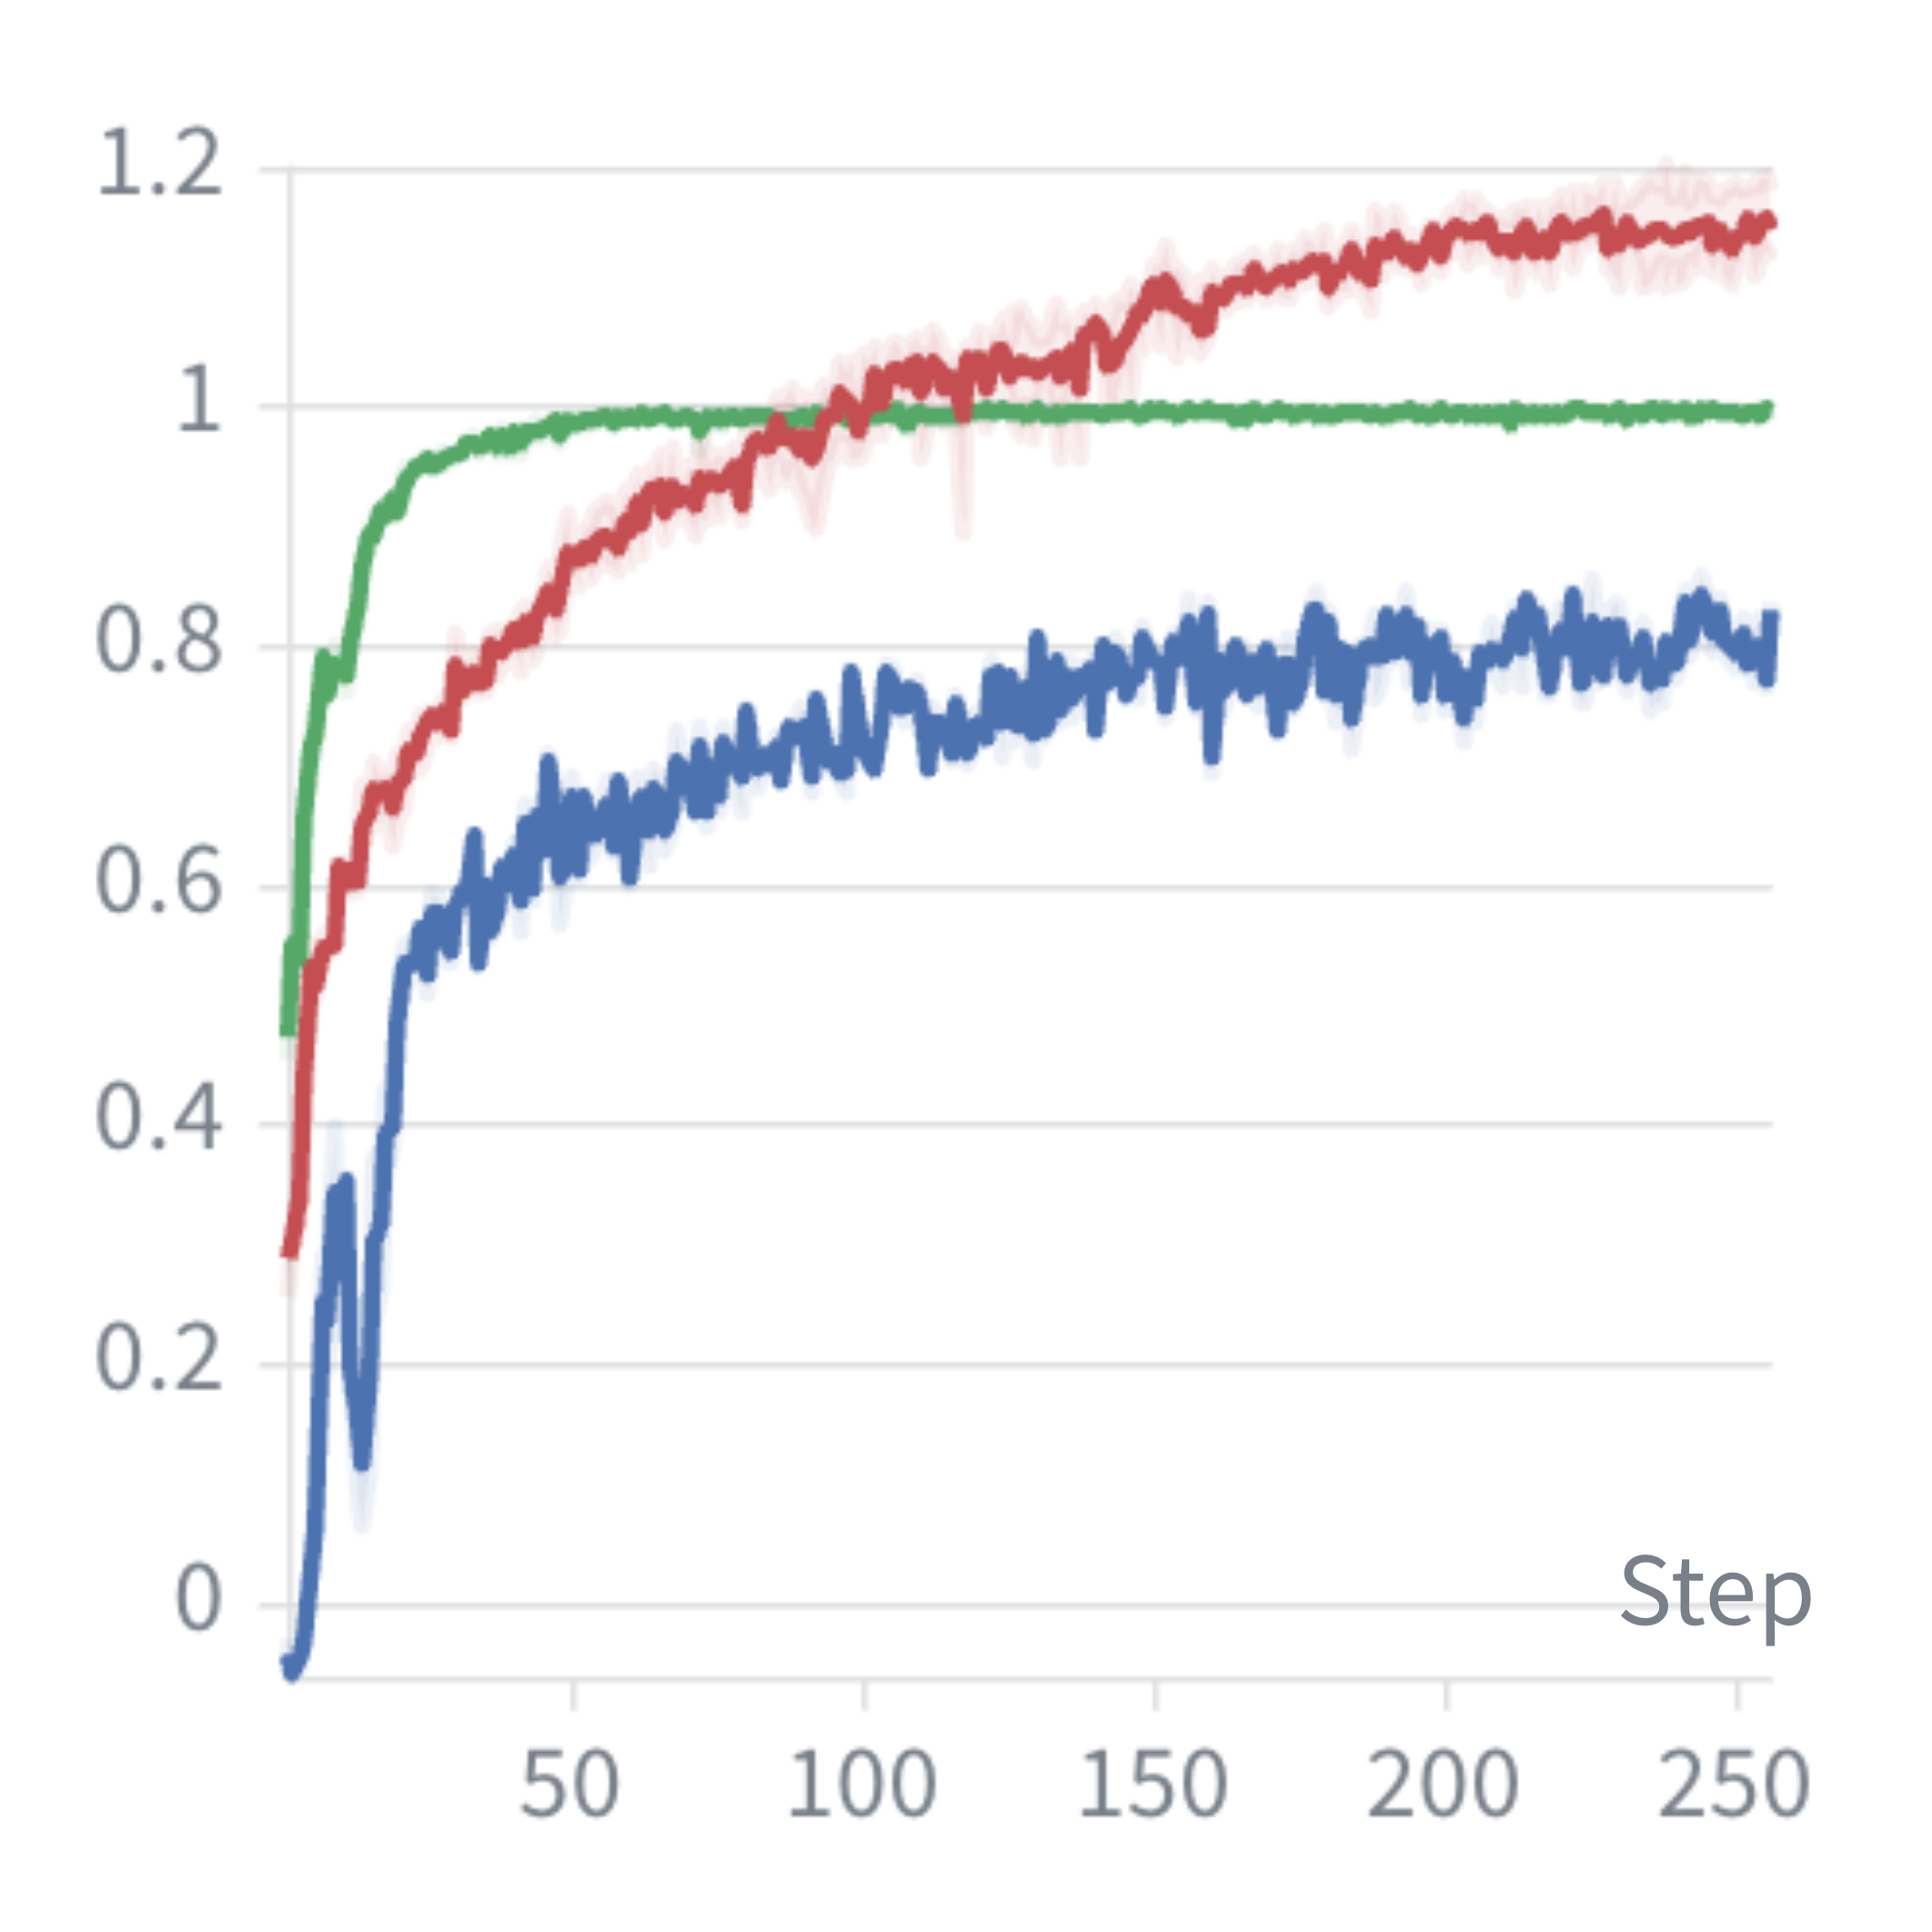
\includegraphics[width=\linewidth]{figures/vlmarch-reward-2.png}
%     \end{subfigure}
%     \caption{Training dynamics of \ours, showing the entropy convergence (left) and reward curve (right) across training iterations.
%     % selfcheck 是指 response-level self-verification 的对比方法，使用图像和模型回复进行整体的自我验证。
%     % selfcheck(GT) 是指 response-level self-verification 的对比方法，使用了GQA中提供的ground truth和模型回复进行整体自我验证。
%     }
%     \label{fig:training-dynamics}
% \end{figure}

% %% overhead数据
% % Ours 的方法每一个training step用时 281.21 s，agent个数为4次
% % selfcheck 方法用时 180.02 s，single agent
% % selfcheck(GT) 方法用时 171.24 s, single agent
% % agent数量 x4, 训练时间 x1.56

% Figure~\ref{fig:training-dynamics} illustrates the entropy and reward curves of \ours alongside two response-level baselines—\textit{SelfCheck}, which verifies the full response against the image, and \textit{SelfCheck (GT)}, which verifies against ground-truth annotations—over 250 training steps.

% \textbf{Entropy.}
% \ours exhibits a rapid and sustained entropy reduction, converging to near-zero by step 50 and remaining stable throughout training.
% In contrast, both SelfCheck variants maintain substantially higher entropy (${\approx}0.75$--$0.85$) with visible oscillations, indicating that holistic response-level signals fail to provide a sufficiently precise reward for the model to commit to a stable output distribution.
% The sharp entropy collapse of \ours reflects that claim-level verification supplies unambiguous, fine-grained feedback that effectively guides policy optimization toward deterministic and well-calibrated responses.

% \textbf{Reward.}
% Correspondingly, \ours achieves the highest final reward (${\approx}1.15$) among all three methods, with a smooth and monotonic ascent after an initial warm-up phase.
% SelfCheck plateaus early at ${\approx}1.0$, while SelfCheck (GT)—despite having access to ground-truth labels—saturates at a lower level (${\approx}0.8$), suggesting that coarse binary supervision from ground truth is less informative than the structured multi-step verification signal in \ours.
% The continued reward growth of \ours beyond step 150, where baselines have already plateaued, further demonstrates the superiority of claim-level granularity in sustaining learning progress.

% \textbf{Computational Overhead.}
